% Aqui começa o capítulo de Introdução.
% Use o comando \label para definir um rótulo, 
% caso seja necessário referenciar esse capítulo
% posteriormente.
\chapter{Introdução}\label{chp:Introducao}

% O comando a seguir gera um "dummy text". 
% Elimine-o quando escrever sua dissertação.
\lipsum[1]

Aqui um exemplo de como referenciar a \Tabela{tab:tabela_1}. Note que é preciso definir um rótulo (\textit{label}) dentro do comando de definição da tabela.

% Veja a seguir um exemplo de Tabela.
% Você pode usar o site http://www.tablesgenerator.com
% para gerar as tabelas em LaTeX.
\begin{table}[!htp]
\caption[Legenda curta da tabela]{Legenda longa e mais detalhada da tabela.}
\label{tab:tabela_1}
\begin{center}
\begin{tabular}{|c|c|}
\hline
Coluna 1 & Coluna2 \\ \hline\hline
a & b \\\hline
c & d \\\hline
\end{tabular}
\end{center}
\end{table}

As tabelas mais complexas podem ser feitas com ajuda no site \href{http://www.tablesgenerator.com}{http://www.tables\-ge\-ne\-ra\-tor.com}.

Veja um exemplo de equação no próprio texto, e.g., $x=\frac{\sqrt[y]{a^{2}+b^{2}}}{\sigma}$.  Se você preferir, pode escrever a equação de forma estendida, conforme a \Equacao{eq:teste} a seguir. Note que o rótulo é colocado automaticamente.

\begin{equation}
x=\frac{\sqrt[y]{a^{2}+b^{2}}}{\sigma}
\label{eq:teste}
\end{equation}

Você também pode obter ajudar para escrever as equações em \LaTeX no site \url{http://www.codecogs.com/latex/eqneditor.php}.

Note que podemos incluir automaticamente alguns termos na lista de símbolos no pré-texto. Veja exemplos a seguir no código fonte. Eles não aparecerão no arquivo gerado. 

\nomenclature{$a$}{Valor obtido a partir de um termo}%
\nomenclature{$b$}{Outro valor obtido a partir de outro termo}%

Veja na \Secao{sec:exemplo_secao} a seguir como referenciar uma seção. Também será preciso definir um rótulo (\textit{label}) logo após o comando \texttt{$\backslash$section}.

% Aqui começa uma Seção.
% Use o comando \label para definir um rótulo, 
% caso seja necessário referenciar essa seção
% posteriormente.
\section{Exemplo de seção}\label{sec:exemplo_secao} 
Agora observe como se faz uma citação de artigo científico em periódico \cite{Gradvohl2014c}. De acordo com \textcite{Gradvohl2016}, essa é uma citação direta. Se for citar mais de um trabalho, faça da seguinte forma \cite{ZAMBON2015, Gradvohl2015}. As referências bibliográficas estão no arquivo \texttt{bibliografia.bib}

Veja a seguir o comando para criar uma figura e o resultado, na \Figura{fig:xwing}.

\begin{figure}[!htb]
\centering
%As figuras estão na pasta figuras.
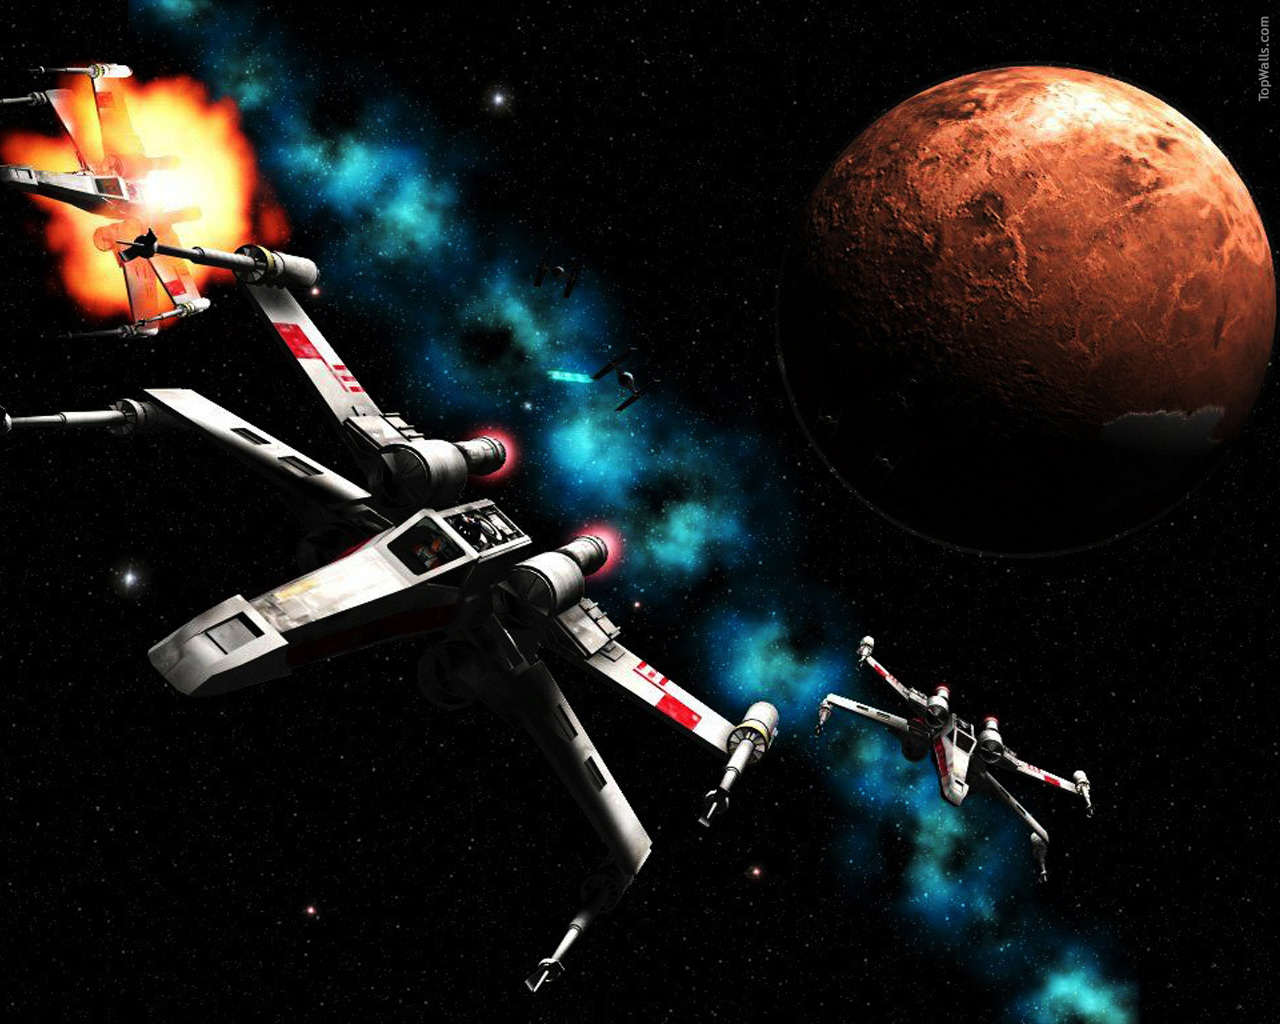
\includegraphics[scale=0.2]{starwars21280.jpg}
\caption[Legenda curta de figura]{Legenda mais extensa de figura.}
\label{fig:xwing}
\end{figure}

\subsection{Exemplo de subseção}
É importante evitar chegar a esse nível de subseção. Dois níveis é suficiente. Use essa opção em último caso, apenas.

% O comando a seguir gera um "dummy text". 
% Elimine-o quando escrever sua dissertação.
\lipsum[5]
